\section{A Machine Model for Line-rate Switches}
\label{s:absmachine}

\begin{figure*}[!t]
  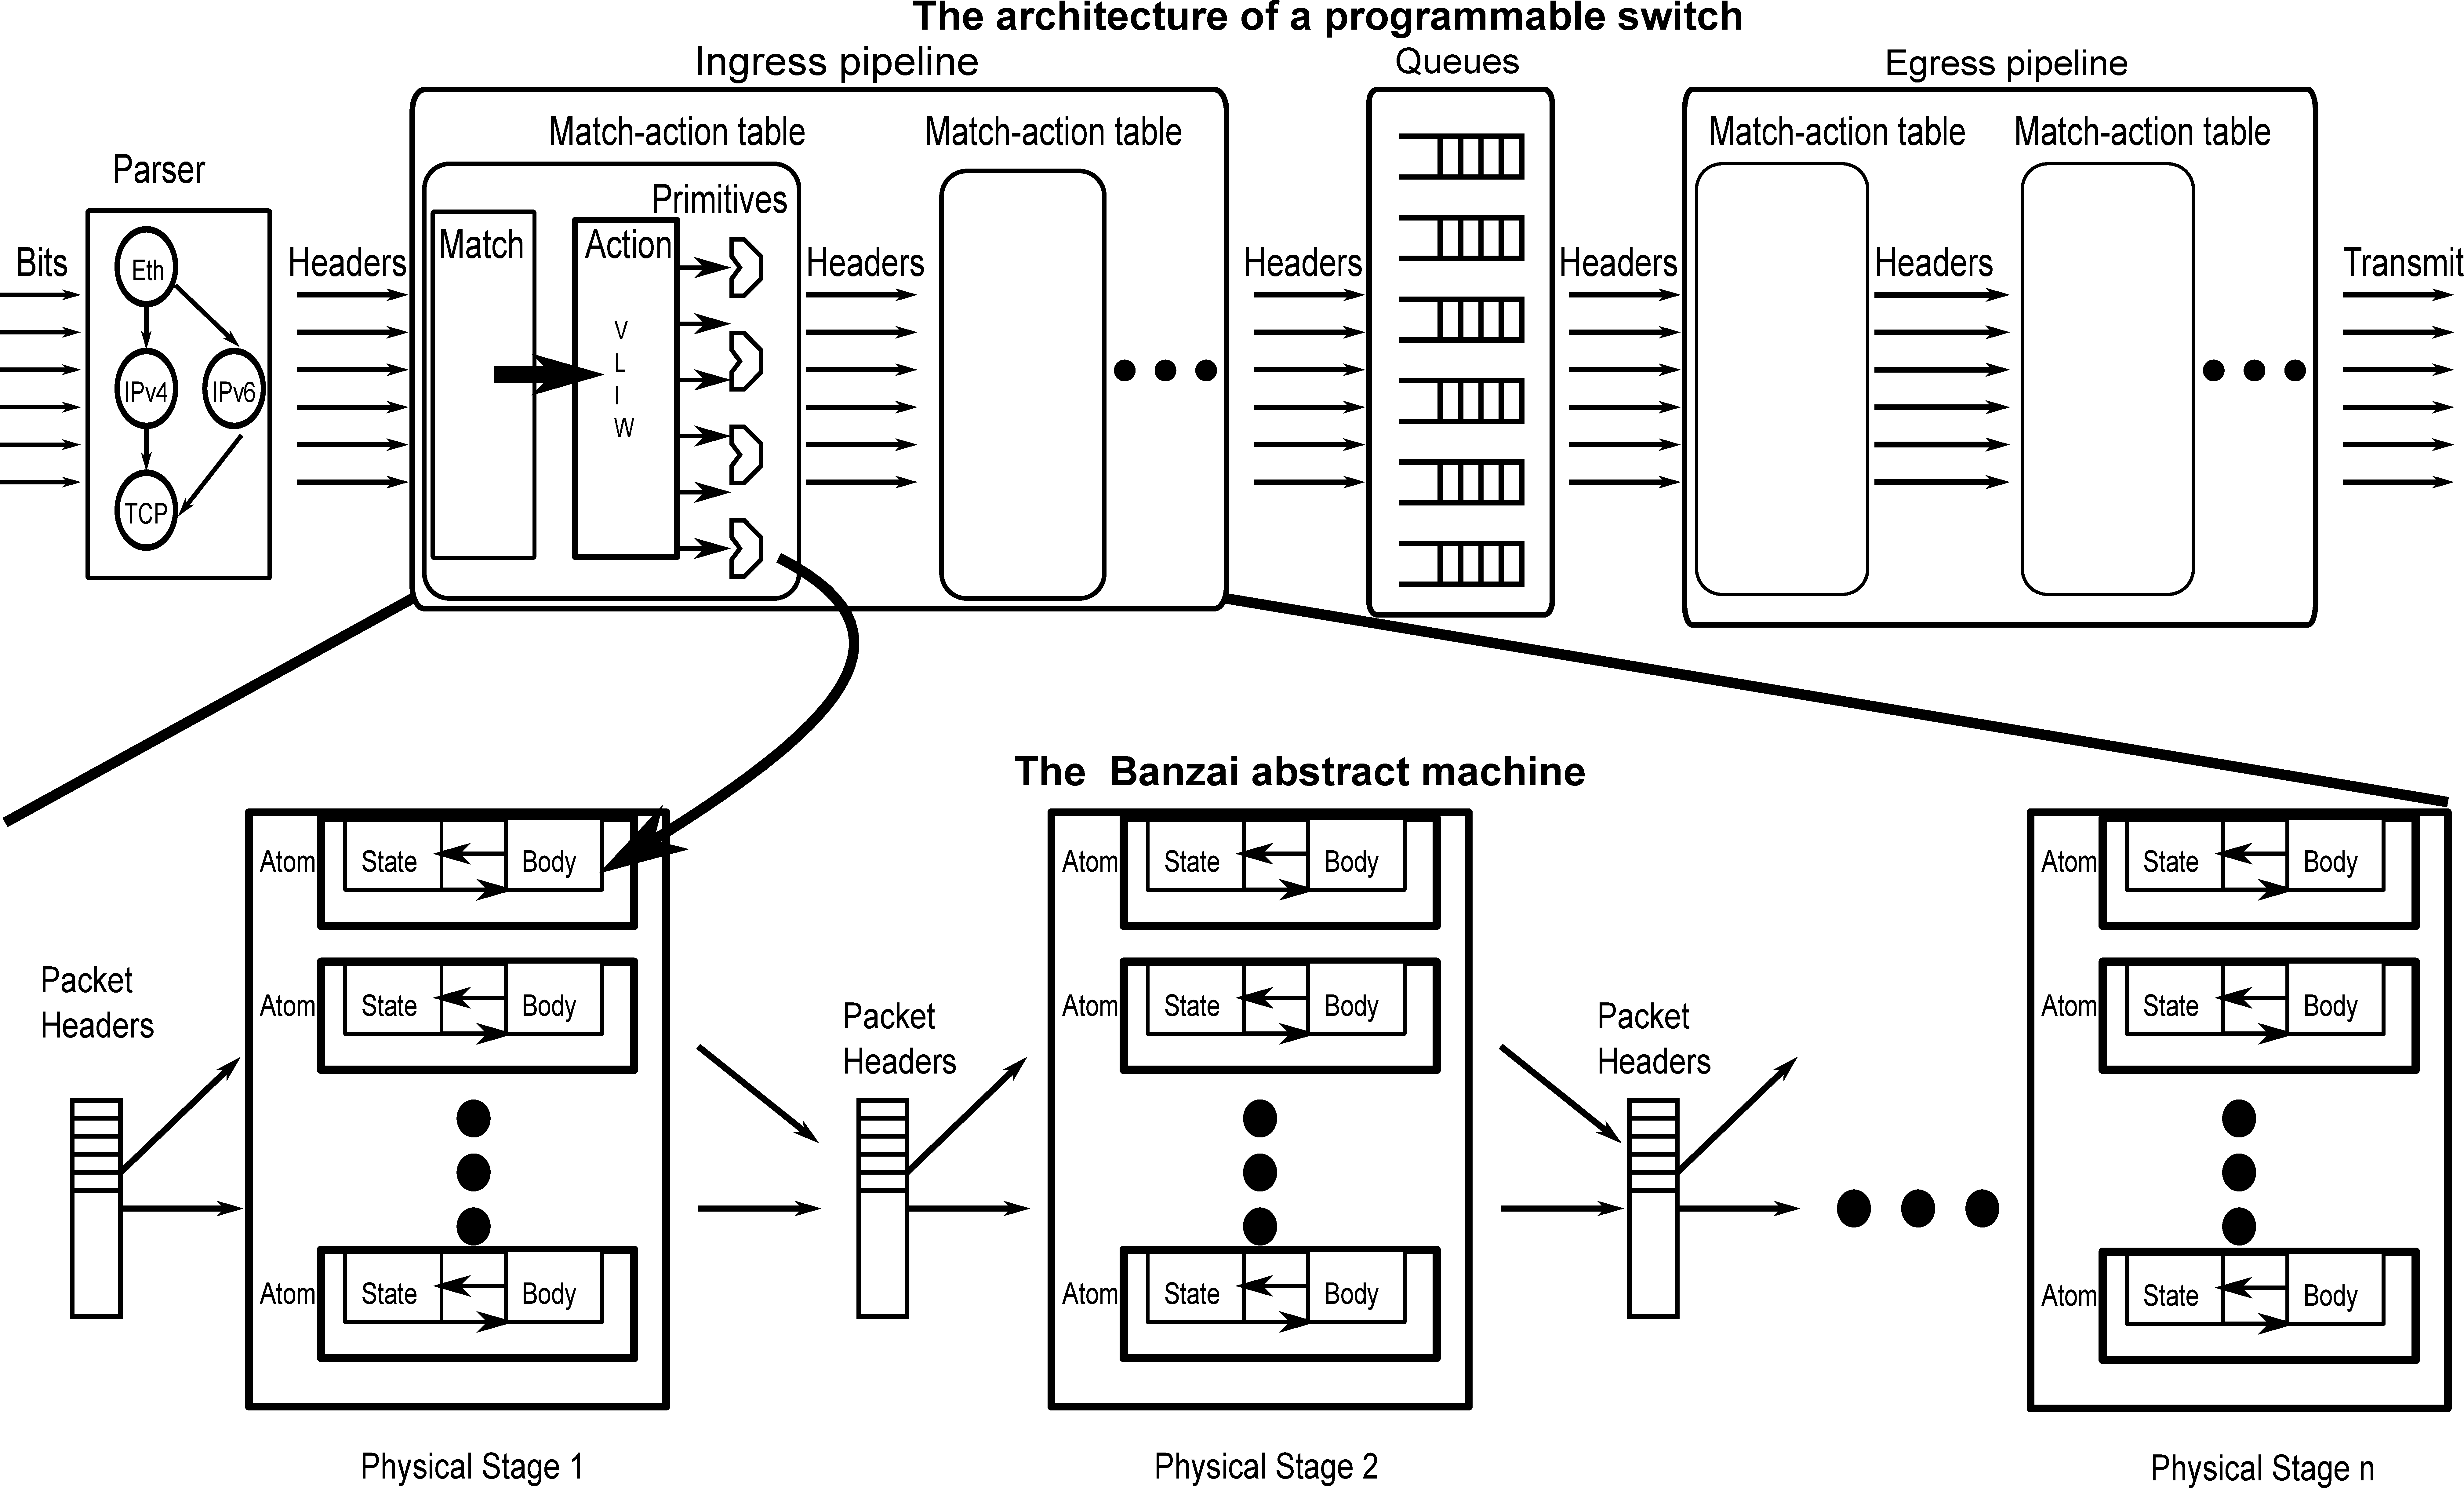
\includegraphics[width=\textwidth]{banzai.pdf}
  \caption{The \absmachine machine model and its relationship to
  programmable switch architectures.}
  \label{fig:switch}
\end{figure*}

\absmachine is a machine model for programmable line-rate switches
that serves as the compiler target for \pktlanguage programs.
\absmachine's design is inspired by recent programmable switch
architectures such as RMT~\cite{rmt}, Intel's
FlexPipe~\cite{flexpipe}, and Cavium's XPliant Packet
Architecture~\cite{xpliant}. \absmachine abstracts these architectures
and extends them with stateful processing units to implement
data-plane algorithms. These processing units, called {\em atoms},
precisely model the set of operations that a hardware target can
execute at line rate; they function as the target instruction set for
the \pktlanguage compiler.

\subsection{Background: Programmable switches}
Packets arriving at a programmable switch~(Figure~\ref{fig:switch}) are parsed
by a programmable parser that turns packets into header fields. These header
fields are first processed by an ingress pipeline consisting of match-action
tables arranged in stages. Processing a packet at a stage may modify its header
fields as well as some persistent state at that stage. Each stage has access
only to its own local state. To share state between stages, it must be carried
forward in packet headers. Following the ingress pipeline, the packet is
queued. Once the packet is dequeued by the switch scheduler, it is processed by
a similar egress pipeline before being transmitted.

To reduce chip area, the ingress and egress pipelines are shared across switch
ports.  Each pipeline handles aggregate traffic belonging to all ports on the
switch, at all packet sizes.  For instance, a 64-port switch with a line rate
of 10 Gbits/s per port and a minimum packet size of 64 bytes needs to process
around a billion packets per second~\cite{rmt}.  Equivalently, with a clock
frequency of 1 GHz, each pipeline stage needs to process one packet every clock
cycle (1 ns).  The need to handle one packet per clock cycle is typical because
switches are designed for the highest port count and line rate for a given chip
area. We assume one packet per clock cycle throughout the paper.\footnote{For
concreteness, we assume a 1 GHz clock frequency.}
%TODO: Define line rate.

Having to process a packet every clock cycle in each stage greatly
constrains the operations that can be performed on each packet. In
particular, any packet operation that modifies state visible to the
next packet {\em must} finish execution in a single clock cycle (see
\S\ref{ss:atoms} for details). Because of this restriction,
programmable switching chips provide a small set of processing units
or primitives for manipulating packets and state in a stage, unlike in
software routers. These processing units determine what algorithms can
run on the switch at line rate.

The challenge here is to determine primitives that allow a broad range of
data-plane algorithms to be implemented, and build a compiler to map a
user-friendly description of an algorithm to the primitives provided by a
switch.

\subsection{The \absmachine machine model}

\absmachine (the bottom half of Figure~\ref{fig:switch}) models the data-plane
components of an ingress or egress switch pipeline, consisting of a number of
stages executing synchronously on every clock cycle. Each stage processes one
packet every clock cycle (1 ns) and hands it off to the next, until it exits
the pipeline. \absmachine models the computation within a match-action table in
a stage (i.e., the action half of the match-action table), but not the match
semantics (e.g., direct, or ternary) (we discuss how to embed these
computations in a standard match-action pipeline in \S\ref{ss:guards}).
\absmachine does not model packet parsing and assumes that packets arriving to
it are already parsed.

\subsection{Atoms: \absmachine's processing units}
\label{ss:atoms}

Each pipeline stage in \absmachine contains a {\em vector of
  atoms}. All atoms in the vector execute in parallel on every clock
cycle.  Informally, an atom is an atomic unit of packet processing
supported natively by a \absmachine machine.
The atoms provided by 
a \absmachine machine form its instruction set.
Atoms may modify persistent state stored on the
switch. In contrast to instruction sets for CPUs, GPUs, DSPs, and
NPUs, the atoms for a \absmachine machine need to be substantially
richer to run real-world data-plane algorithms at line rate. We
explain why with an example.

Suppose we need to atomically increment a state variable stored on the switch
to count packets. One approach would be to have hardware support for three
simple single-cycle operations: \textit{read} some memory in the first clock
cycle, \textit{add} one in the next, and \textit{write} it to memory in the
third. This approach, however, does not provide atomic isolation. To see why,
suppose packet $A$ increments the counter from 0 to 1 by executing the read,
add, and write operations at clock cycles 1, 2, and 3 respectively.  If packet
$B$ issues the read at time 2, it will increment the counter again from 0 to 1,
when it should be 2. Locks over the shared counter are a potential
solution. However, locking causes packet $B$ to wait during packet $A$'s
increment, and the switch no longer sustains line rate of one packet every
clock cycle.\footnote{Wait-free objects~\cite{herlihy_wait} are an alternative
  to locking, but are typically too complex for hardware.} CPUs employ microarchitectural
  techniques such as operand forwarding to address this problem, but these techniques
  suffer from occasional pipeline stalls, which militates against line-rate
  performance.
%% TODO: Not mentioning that shared memory is costly. Because, while that's true.
%% there are parts of the switch pipeline that use it (such as the scheduler).

The only way to provide an atomic increment is to explicitly support it in
hardware with an {\em atom} to read memory, increment it, and write it back in
a single stage within one clock cycle. The same observation applies to any
other line-rate atomic operation.

This observation motivates why we represent an atom as a body of sequential
code. An atom completes execution of the entire body of code and modifies a
packet before processing the next packet.  An atom may also contain internal
state that is local to that atom alone and persists across packets. An atom's
body of sequential code fully specifies the atom's behavior and serves as an
interface between the compiler and the programmable switch hardware.
%%\ac{does this mean we could have invented a new
%%instruction to represent each atom, and the current representation as a
%%body of (C-like?) sequential code is simply convenience for people to 
%%implement different banzai machines?}
%%No. You need someway to represent an atom's functionality to the compiler.
%% like expression trees / tiles for instruction selection.

Using this representation, a switch counter that wraps around at a
value of 100 can be written as the atom:\footnote{We use {\tt p.x} to
  represent field {\tt x} within a packet {\tt p} and {\tt x} to
  represent a state variable {\tt x} that persists across packets.}
\begin{lstlisting}[style=customc, numbers=none, frame=none]
if (counter < 99)
  counter++;
else
  counter = 0;
\end{lstlisting}
Similarly, a stateless operation like setting a packet field
(e.g. P4's {\tt modify\_field} primitive~\cite{p4spec}) can be written
as the atom:
\begin{lstlisting}[style=customc, numbers=none, frame=none]
  p.field = value;
\end{lstlisting}
Table~\ref{tab:templates} provides more examples of atoms.

We note that---unlike stateful atomic operations such as a counter---stateless
atomic operations are easier to support with basic packet-field arithmetic.
Consider, for instance, the operation {\tt pkt.f1 = pkt.f2 + pkt.f3 - pkt.f4}.
This operation does not modify any persistent switch state because it only
reads and writes packet fields. It can be implemented without violating
atomicity by using two atoms: one atom to add fields f2 and f3 in one pipeline
stage (clock cycle), and another to subtract f4 from the result in the
next---without having to provide one large atom that supports the entire
operation.

%%\ac{but I thought you are still implement the whole thing as one single atom
%%right? What's the point here}
%% The point is we can implement this as two atoms without violating atomicity.
%% Explained above.

\subsection{Constraining atoms}
\label{s:atomConstraints}

\textbf{Computational limits:} To provide line-rate performance, atom
bodies must finish execution within one clock cycle. We
constrain atom bodies by defining {\it atom templates}
(\S\ref{ss:code_gen}).  An atom template is a program that always
terminates and specifies exactly how the atom is executed. One example
is an ALU with a restricted set of primitive operations to choose from
(Figure~\ref{fig:alu_diag}). Atom templates allow us to create
\absmachine machines with different atoms.  In practice, atom
templates will be designed by an ASIC engineer and exposed as a
machine's instruction set~(\S\ref{ss:targets}).  As programmable
switches evolve, we expect that atoms will evolve as well, but
constrained by the clock-cycle requirement~(\S\ref{ss:perfprog}).

\begin{figure}[h]
  \begin{subfigure}{0.4\columnwidth}
  \begin{center}
  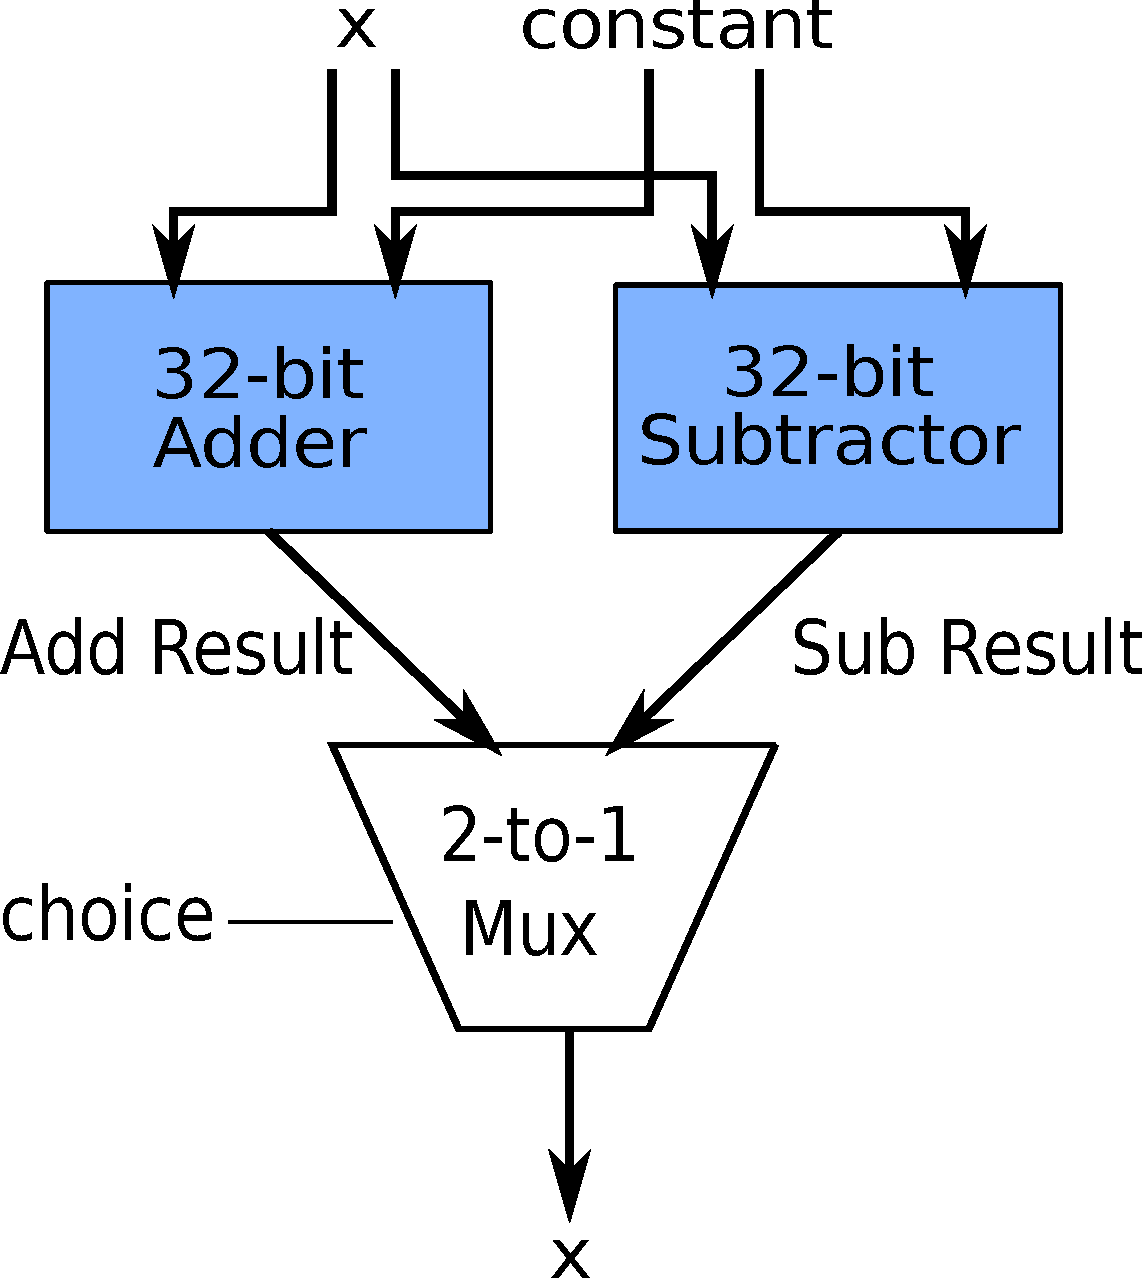
\includegraphics[width=\columnwidth]{circuit.pdf}
  \end{center}
  \caption{Circuit for an atom that can add or subtract a constant from a state variable.}
  \label{fig:alu_diag}
  \end{subfigure}
  \hspace{0.05\columnwidth}
  \begin{subfigure}{0.55\columnwidth}
  \begin{lstlisting}
  bit choice = ??;
  int constant = ??;
  if (choice) {
    x = x + constant;
  } else {
    x = x - constant;
  }
  \end{lstlisting}
  \caption{Circuit representation as an atom template.}
  %Each ``??(n)'' represents a hole that can be filled in with values in $[0, 2^n -1]$.}
  \label{fig:alu_in_sketch}
  \end{subfigure}
  \caption{Atoms and atom templates}
  \label{fig:atom}
\end{figure}

\textbf{Resource limits:} For any real machine, we also need to limit the
number of atoms in each stage (\textit{pipeline width}) and the number of
stages in the pipeline (\textit{pipeline depth}). This is similar to limits on
the number of stages, number of tables per stage, and amount of memory per
stage in programmable switch architectures such as RMT and
FlexPipe~\cite{lavanya_compiler}.

\subsection{What can \absmachine not do?}
\label{ss:limitations}

Like real programmable switches, \absmachine is a good fit for data-plane
algorithms that modify a small set of packet headers and carry out small
amounts of stateful or stateless computation per packet. Data-plane algorithms
like deep packet inspection and WAN optimization require a switch to parse and
process the packet payload as well---effectively parsing a large ``header''
consisting of each byte in the payload, which is challenging at line rates of 1
GHz. Such algorithms are best left to general-purpose CPU platforms~\cite{e2,
aplomb, opennf}. Some algorithms require complex computations, but not on every
packet.  For example, consider a measurement algorithm that periodically scans
a large table to perform garbage collection.  \absmachine's atoms model small
computations that occur on every packet, and are not suitable for such
operations that span many clock cycles.
